\chapter{Electronic Excited States}

\graphicspath{{./Figures/ExcitedStates/}}

\section{Introduction}
Most of the discussion of quantum chemical calculations thus far has
centered on ground state properties. Quantum chemical techniques can
also be used to compute energies and wave functions for electronically
excited states.

Excited states are most relevant when considering absorption
spectroscopy. Molecules can absorb a photon in the Vis-UV range and
convert to an electronically excited state. 
Koopman's theorem suggests that the orbital energies for the orbitals
approximate the energy required to ionize an electron from that
orbital. We can also use the orbital energies to approximate the
excitation process between two orbitals.

\begin{figure}
\begin{center}
\includegraphics[scale=0.6]{koopman-excite}
\end{center}
\caption{Orbital energies approximating the excitation energy between
two orbitals. The HOMO--LUMO excitation shown would have an excitation energy $E_j-E_i$.} 
\label{koopman-excite}
\end{figure}

Figure \ref{koopman-excite} shows how the orbital energies may be used
approximate excitation energies.

There is one problem with using orbital energies in this fashion. The
orbital energies of the virtual (unoccupied) orbitals actually
corresponds to the states that contain an additional electron. The
orbital energies are computed from interactions where a particle in
the virtual orbitals sees all of the $N_{el}$ electrons, whereas in
reality it should only see $N_{el}-1$ electrons, since it shouldn't
see itself.

\begin{figure}
\begin{center}
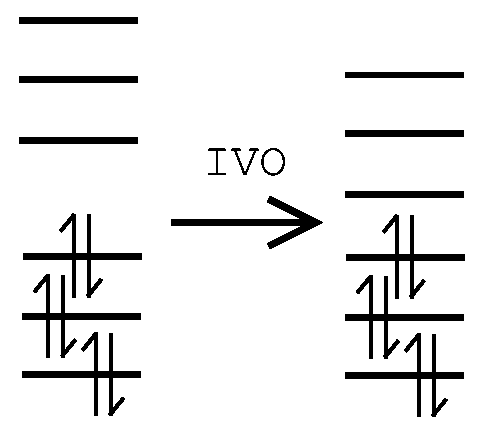
\includegraphics[scale=0.6]{ivo.eps}
\end{center}
\caption{IVO treatment leads to more realistic virtual orbitals and
orbital energies.}  
\label{ivo}
\end{figure}

We can correct this difficulty by using \emph{improved virtual
orbitals} (IVOs). IVOs keep the normal set of occupied orbitals, but
use the state with $N_{el}-1$ electrons for the virtual
orbitals. These orbitals and the associated orbital energies much more
accurately reproduce the proper excited state energies. Figure
\ref{ivo} shows schematically the effect of the ivo treatment.

The following sections detail more rigorous techniques for computing
excited states.

\section{Open Shell Singlet Calculations}
An open-shell singlet (OSS) state is very similar to a triplet state,
except that the two orbitals are singlet paired rather than triplet
paired. A triplet pairing is given by
\begin{equation}
 \Psi_{T} = \phi_{core}\phi_a\phi_b\alpha\alpha
\end{equation}
whereas the open-shell singlet wave function is given by
\begin{equation}
 \Psi_{OSS} = \phi_{core}(\phi_a\phi_b+\phi_b\phi_a)
  (\alpha\beta-\beta\alpha).
\end{equation}
The energy for the triplet wave function is given by $E_{core} +
J_{ab} - K_{ab}$, and the energy of the OSS wave function is given by
$E_{core} + J_{ab} + K_{ab}$.  

OSS wave functions are convenient because they allow standard grand
state programs to be used to compute excited state energies and wave
functions. 

\section{Configuration Interaction Singles}
Open shell singlet descriptions are limited to excited states that can
be described as a single excitation process. Most excited states fall
into this category, but not all do. For those states we may use a
single-excitation configuration interaction approach. Consider a
molecule with occupied orbitals $\phi_a$, $\phi_b$, $\phi_c$,
$\phi_d$, and virtual orbitals $\phi_r$, $\phi_s$, $\phi_t$,
$\phi_u$, and ground state wave function $\Psi$. We write the singly
excited state (also known as a singly excited determinant) when we
take an electron out of occupied orbital $\phi_a$ and put it into
virtual orbital $\phi_r$ as $\Psi_a^r$. We can approximate the excited
state wave function as a linear combination of all of these excited
configurations
\begin{eqnarray}
 \Psi_{CIS} &=& \Psi_a^r + \Psi_a^s + \Psi_b^r + \Psi_b^s + \dots \\
            &=& \sum_i^{occ}\sum_m^{virt} a_{im}\Psi_i^m.
\end{eqnarray}
We wish to find the most optimal linear combination, the one with the
lowest energy. We determine this by forming the Configuration
Interaction (CI) matrix, 
\begin{eqnarray}
 A_{im,jn} = \bracket{\Psi_i^m}{H}{\Psi_j^n}.
\end{eqnarray}
The CI matrix is huge: for a molecule with $n_o$ occupied orbitals and
$n_v$ virtual orbitals, there are $n_o^2n_v^2$ elements, which means
that forming and diagonalizing the matrix can become computationally
expensive very quickly. Typically, only a small range of orbitals
close to the HOMO and LUMO are used as the \emph{active space}, since
realistically, these are the only orbitals that participate in the
excited state to an appreciable degree.

%\section{Time Dependent HF and DFT}

\section{Comparison of results for test systems}
Table \ref{excited} presents results for the methods discussed in this
chapter for a few small molecules whose vertical excitation energies
were well studied experimentally.

\begin{table}
\caption{Vertical excitation energies (in kcal/mol) for a few small
molecules, computed using the techniques discussed in this chapter,
along with experimental results. Computations are performed using the
6-31G** basis set.}
\label{excited}
\begin{center}
\begin{tabular}{cccccc}\hline\hline
Molecule & $\Delta E$ Koopman &  $\Delta E$ IVO &  $\Delta E$ OSS &
  $\Delta E$ CIS &  $\Delta E$ Exp.\\ \hline
Ethylene        & 394.84 & 171.93 & 224.88 & 207.63 & 163.96 \\
Formaldehyde    & 363.90 & 146.65 & 79.25  & 109.92 & 80.71 \\
cis-Butadiene   & 294.21 & 149.87 & 168.15 & 161.67 & 126.60 \\
trans-Butadiene & 285.12 & 144.96 & 173.27 & 165.55 & 136.62 \\
\hline\hline
\end{tabular}
\end{center}
\end{table}

% RPM: repeat table with larger basis?

\section{Nonlinear optical properties of molecules}
Molecules are polarizable: when we put them into an electric field
their electrons reorganize. We can use the dipole moment as a way of
monitoring this polarization
\begin{equation}
 \mu = \mu_0 \alpha E + \frac{\beta E^2}{2!} + \frac{\gamma E^3}{3!} +
  \dots
\label{dipole-nlo}
\end{equation}
The term $\alpha$ is the linear polarizability, $\beta$ is the first
hyperpolarizability, and $\gamma$ is the second
hyperpolarizability. Nonlinear optical effects such as frequency
doubling and second-harmonic generation are a property primarily of
the first hyperpolarizability, so computing this effect efficiently is
of great interest to us.

\begin{figure}
\begin{center}
\includegraphics[scale=0.5]{polymer_nlo.eps}
\end{center}
\caption{Two valence bond extremes used to model the polarization
process in a conjugated polymer.}
\label{polymer_nlo}
\end{figure}

Figure \ref{polymer_nlo} shows a two-state model for the polarization
process in a conjugated polymer. Here we consider one neutral valence
bond structure ($g$, for the ground state), and one fully charge
transferred valence bond structure ($e$, for the excited state). Using
the excited state, we can approximate the hyperpolarizability as
\begin{equation}
 \beta \approx \frac{\mu_{ge}^2(\mu_{ee}-\mu_{gg})}{E_{ge}^2}.
\end{equation}
That is, the further apart the two states are, the harder it is to
polarize the molecule. Marder, Perry, and coworkers determined that
the bond-length alternation was a good indication of how far apart in
energy the two states were for conjugated polymers, and based design
of NLO materials on this property.

However, we might wish to determine NLO terms like $\beta$ directly.
The finite field technique computes the dipole moment $\mu(\vec{E})$
at a number of different field strengths and orientations, and use
equation (\ref{dipole-nlo}) to fit the values of $\alpha$, $\beta$,
etc., that reproduce these data. This is a good technique, but
requires many different values of the electric to obtain a good fit.

A better technique, when it is available, is to use \emph{Coupled
Perturbed Hartree Fock} (CPHF) techniques. CPHF computes analytical
derivatives of the energy $\frac{\partial E}{\partial X}$, 
$\frac{\partial^2 E}{\partial X\partial Y}$, etc., with respect to the
electric field strength $\vec(E)$ directly. First derivatives are used
to compute the dipole moment, second derivatives are used to compute
the polarizability, and third and higher derivatives are used to
compute the hyperpolarizabilities. Effectively, in the finite
field technique we are approximating these derivatives. However, the
availablility of this method is dependent upon whether the relevant
analytic derivatives have been programmed for the appropriate
Hamiltonian. 

\section{Suggestions for Further Reading}
Hunt and Goddard \cite{Hunt69} discuss IVO calculations. Szabo and
Ostlund \cite{Szabo82} have a good interaction to CI.  CPHF is
discussed in more detail in \emph{A New Dimension to Quantum
Chemistry} \cite{Yamaguchi94}.



